\section{DeepFool attack}

\begin{frame}{DeepFool attack}
    \begin{itemize}
        \item \textbf{Title:} DeepFool: a simple and accurate method to fool deep neural networks (CVPR 2016)
        \item \textbf{Author:} Seyed-Mohsen Moosavi-Dezfooli, Alhussein Fawzi, Pascal Frossard
        % \item \textbf{Contribution}
    \end{itemize}
\end{frame}

\begin{frame}{DeepFool attack}
    文中对抗扰动的定义 : 形式上,对于给定的分类器,对抗扰动则是足以改变预测标签$\hat{k}(x)$的最小扰动,满足
    \begin{equation}
        \begin{aligned}
            \Delta(\boldsymbol{x};\hat{k})
            :=\mathop{\min}\limits_{\boldsymbol{r}}||\boldsymbol{r}||_2  
            \text{ subject to } 
            \hat{k}(\boldsymbol{x}+\boldsymbol{r})\neq \hat{k}(\boldsymbol{x})
          \end{aligned}
    \end{equation}
    $\hat{k}(x)$是原始图像$\boldsymbol{x}$的预测标签, $\Delta(\boldsymbol{x};\hat{k})$是$\boldsymbol{x}$在$\hat{k}$上的鲁棒性。
\end{frame}

\begin{frame}{对于二分类器DeepFool attack}
    \begin{multicols}{2}
        分类标签 $\hat{k}(x)=sign(f(x))$ ,$f(x)$ 是一个图像分类函数,分类边界 $\mathscr{F}\triangleq\{x:f(x)=0\}$ 的两边分别是正负类。
        \begin{figure}
            \centering
            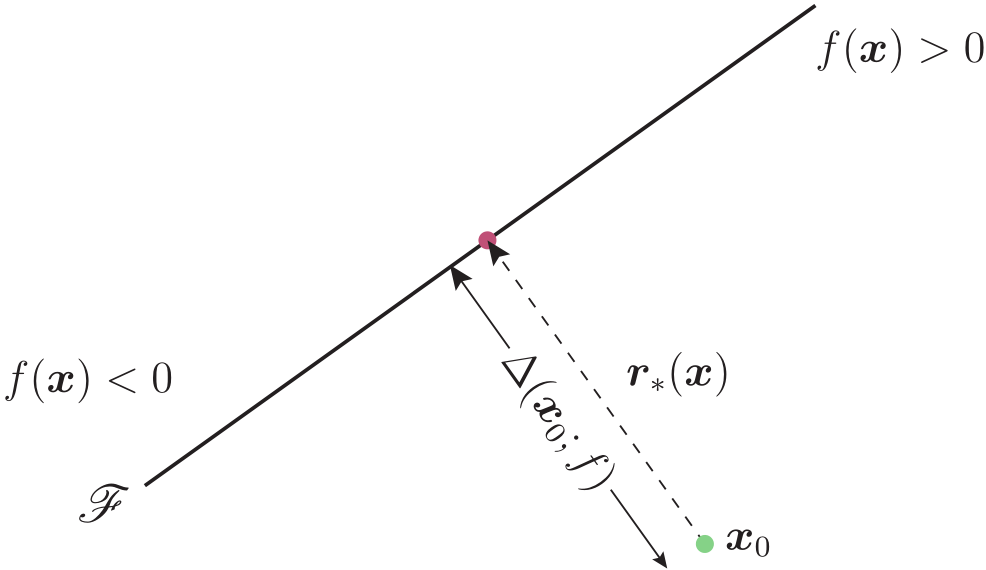
\includegraphics[width=0.3\textwidth]{docs/paperReading/deepfool/deepfool-adv_example_in_linear_classifier.png}
        \end{figure}

        仿射分类器 $f(x)=\omega^T x+b$ 在 $x_0$ 的鲁棒性 $\Delta(x_0;f)$ 等于从 $x_0$ 到仿射超平面 $\mathscr{F}=\{x:\omega^T x+b=0\}$ 的距离

        改变分类器决策的最小扰动 $r_*(x_0)$ 是 $x_0$ 在分类边界 
        $\mathscr{F}$ 上的正交投影:
        \begin{equation}
            \begin{aligned}
                r_*(x_0)    &:=argmin ||r||_2 \\
                            &\text{subject to } sign(f(x_0+r))\neq sign(f(x_0)) \\
                            &=-\frac{f(x_0)}{||\omega||_2^2}\omega
            \end{aligned}
        \end{equation}
    \end{multicols}
\end{frame}

\begin{frame}{对于二分类器DeepFool attack}
    \begin{multicols}{2}
        假设 $f$ 是一个通用的可微的二分类器,采用迭代程序来估计鲁棒性 $\Delta(x_0;f)$ :

        每次迭代中,$f$ 会在当前点 $x_i$ 周围被线性化,线性化分类器的最小扰动为P
        \begin{equation}
            \begin{aligned}
                & argmin_{r_i} ||r_i||_2 \\
                & \text{ subject to } f(x_i)+\nabla f(x_i)^T r_i=0
            \end{aligned}
        \end{equation}
        第 $i$ 轮迭代的扰动 $r_i$ 可以用 $r_*(x_0)$ 计算得出,并且更新下一轮的 $x_{i+1}$ ,直到 $x_{i+1}$ 的符号改变为止

        程序的算法如下:
        \begin{figure}
            \centering
            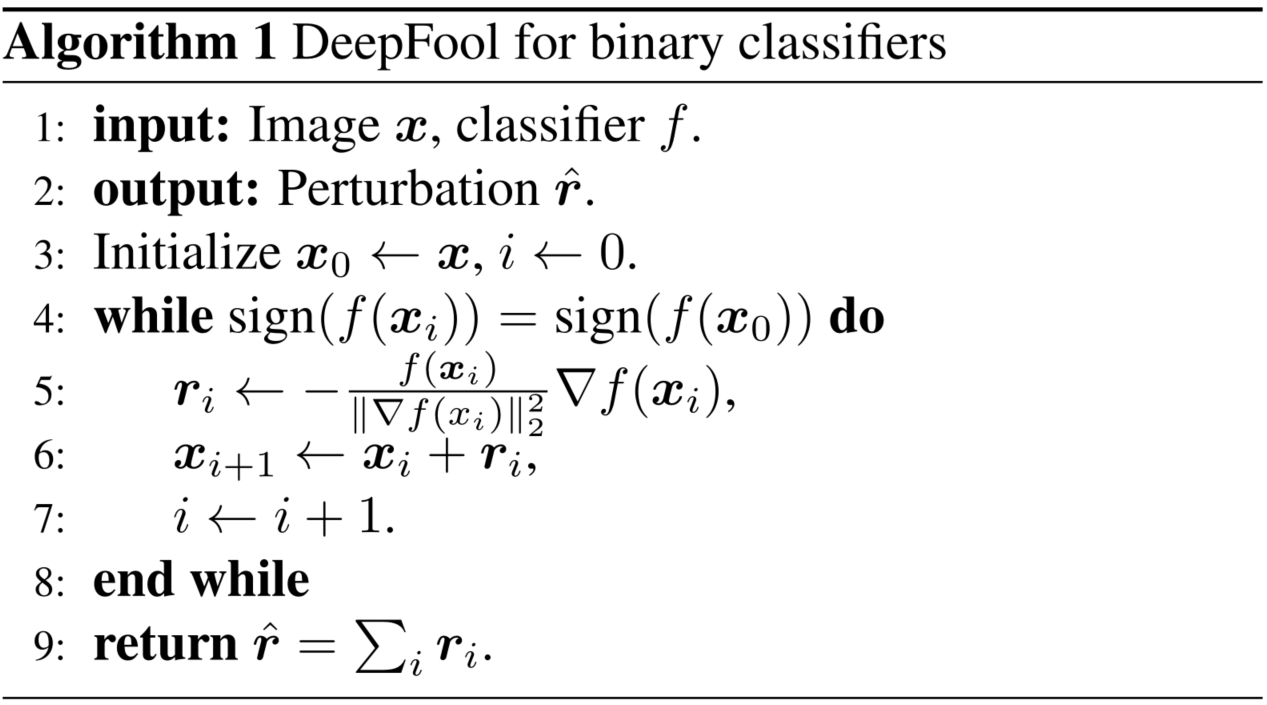
\includegraphics[width=0.7\textwidth]{docs/paperReading/deepfool/deepfool-algorithm_1.png}
        \end{figure}
    \end{multicols}
\end{frame}

\begin{frame}{对于多分类器DeepFool attack}
    多分类器有$c$个分类输出,定义为 $f:\mathbb{R}^n\rightarrow R^c$,分类通过下面映射完成
    \begin{equation}
        \begin{aligned}
            \hat{k}(x)=argmax_{k} f_k(x)
        \end{aligned}
    \end{equation}
    其中 $f_k(x)$ 是与第$k$个类相对应的 $f(x)$ 的输出

    仿射分类器$f(x)$对于给定的$W$和$b$有$f(x)=W^Tx+b$,映射$\hat{k}$是“一对多”的分类,欺骗分类器的最小扰动可以重写为
    \begin{equation}
        \begin{aligned}
            & argmin_{r} ||r||_2 \\
            & \text{s.t. } \exists k:\omega_k^T (x_0+r)+b_k\geq \omega_{\hat{k}(x_0)}^T(x_0+r)+b_{\hat{k}}(x_0)
        \end{aligned}
    \end{equation}
    $\omega_k$ 是$W$的第$k$列。要改变分类结果,必须保证存在一个非原始类标的分类器结果大于原始分类函数的结果
\end{frame}



\begin{frame}{对于多分类器DeepFool attack}
    \begin{multicols}{2}
        多面体 $P$ 定义了输出标签$\hat{k}(x_0)$的空间区域,$x_0$ 在凸多面体 $P$ 内部
        \begin{equation}
            \begin{aligned}
                P=\bigcap_{k=1}^c \{x:f_{\hat{k}(x_0)}(x)\geq f_k(x)\}
            \end{aligned}
        \end{equation}

        几何上,上述的问题就是计算 $x_0$ 与凸多面体 $P$ 的距离 $\textbf{dist}(x_0,P^c)$

        \begin{figure}
            \centering
            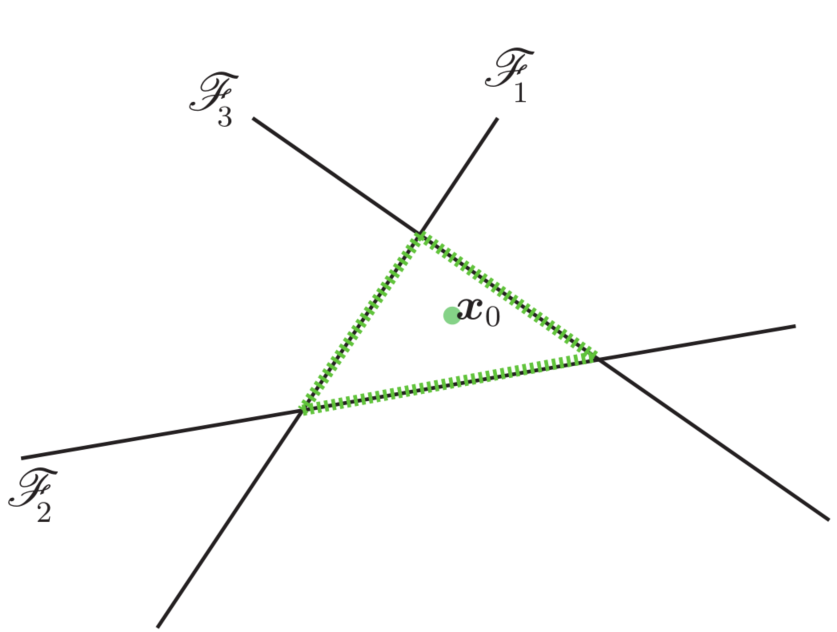
\includegraphics[width=0.3\textwidth]{docs/paperReading/deepfool/deepfool-figure4.png}
        \end{figure}

        例如属于第四类的样本$x_0$,有$\mathscr{F}_k=\{x:f_k(x)-f_4(x)=0\}$,即$x_0$不在$\mathscr{F}_1,\mathscr{F}_2,\mathscr{F}_3$任意一个超平面上。超平面用实线表示,边界$P$用绿线表示
    \end{multicols}
\end{frame}

\begin{frame}{对于多分类器DeepFool attack}
    定义$\hat{l}(x_0)$是距离边界$P$最近的超平面,图中为$\hat{l}(x_0)=3$,$\hat{l}(x_0)$可以计算为
    \begin{equation}
        \begin{aligned}
            \hat{l}(x_0)=argmin_{k\neq \hat{k}(x_0)}\frac{f_k(x_0)-f_{\hat{k}(x_0)}(x_0)}{||\omega_k-\omega_{\hat{k}(x_0)}||_2}
        \end{aligned}
    \end{equation}
    
    最小扰动距离为
    \begin{equation}
        \begin{aligned}
            r_*(x_0)=
            \frac{|f_{\hat{l}(x_0)}(x_0)-f_{\hat{k}(x_0)}(x_0)|}
            {||\omega_{\hat{l}(x_0)}-\omega_{\hat{\hat{k}(x_0)}}||_2^2}  
            (\omega_{\hat{l}(x_0)}-\omega_{\hat{k}(x_0)})
        \end{aligned}
    \end{equation}
    
    也就是说,我们找到了$x_0$在$P$上的最近投影。并且迭代算法也变成
    \begin{equation}
        \begin{aligned}
            P=\bigcap_{k=1}^c 
            \{x:f_{_k}(x_i)-f_{\hat{k}(x_0)}(x_i)+\nabla f_k(x_i)^Tx-\nabla f_{\hat{k}(x_0)}(x_i)^Tx\leq 0\}
        \end{aligned}
    \end{equation}
\end{frame}

\begin{frame}{对于多分类器DeepFool attack}
    程序的算法如下
    \begin{figure}
        \centering
        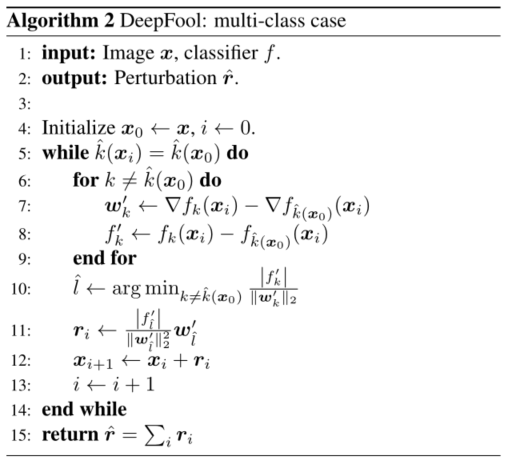
\includegraphics[width=0.46\textwidth]{docs/paperReading/deepfool/deepfool-algorithm_2.png}
    \end{figure}
\end{frame}
\begin{frame}{DeepFool attack实验结果}
    \begin{figure}
        \centering
        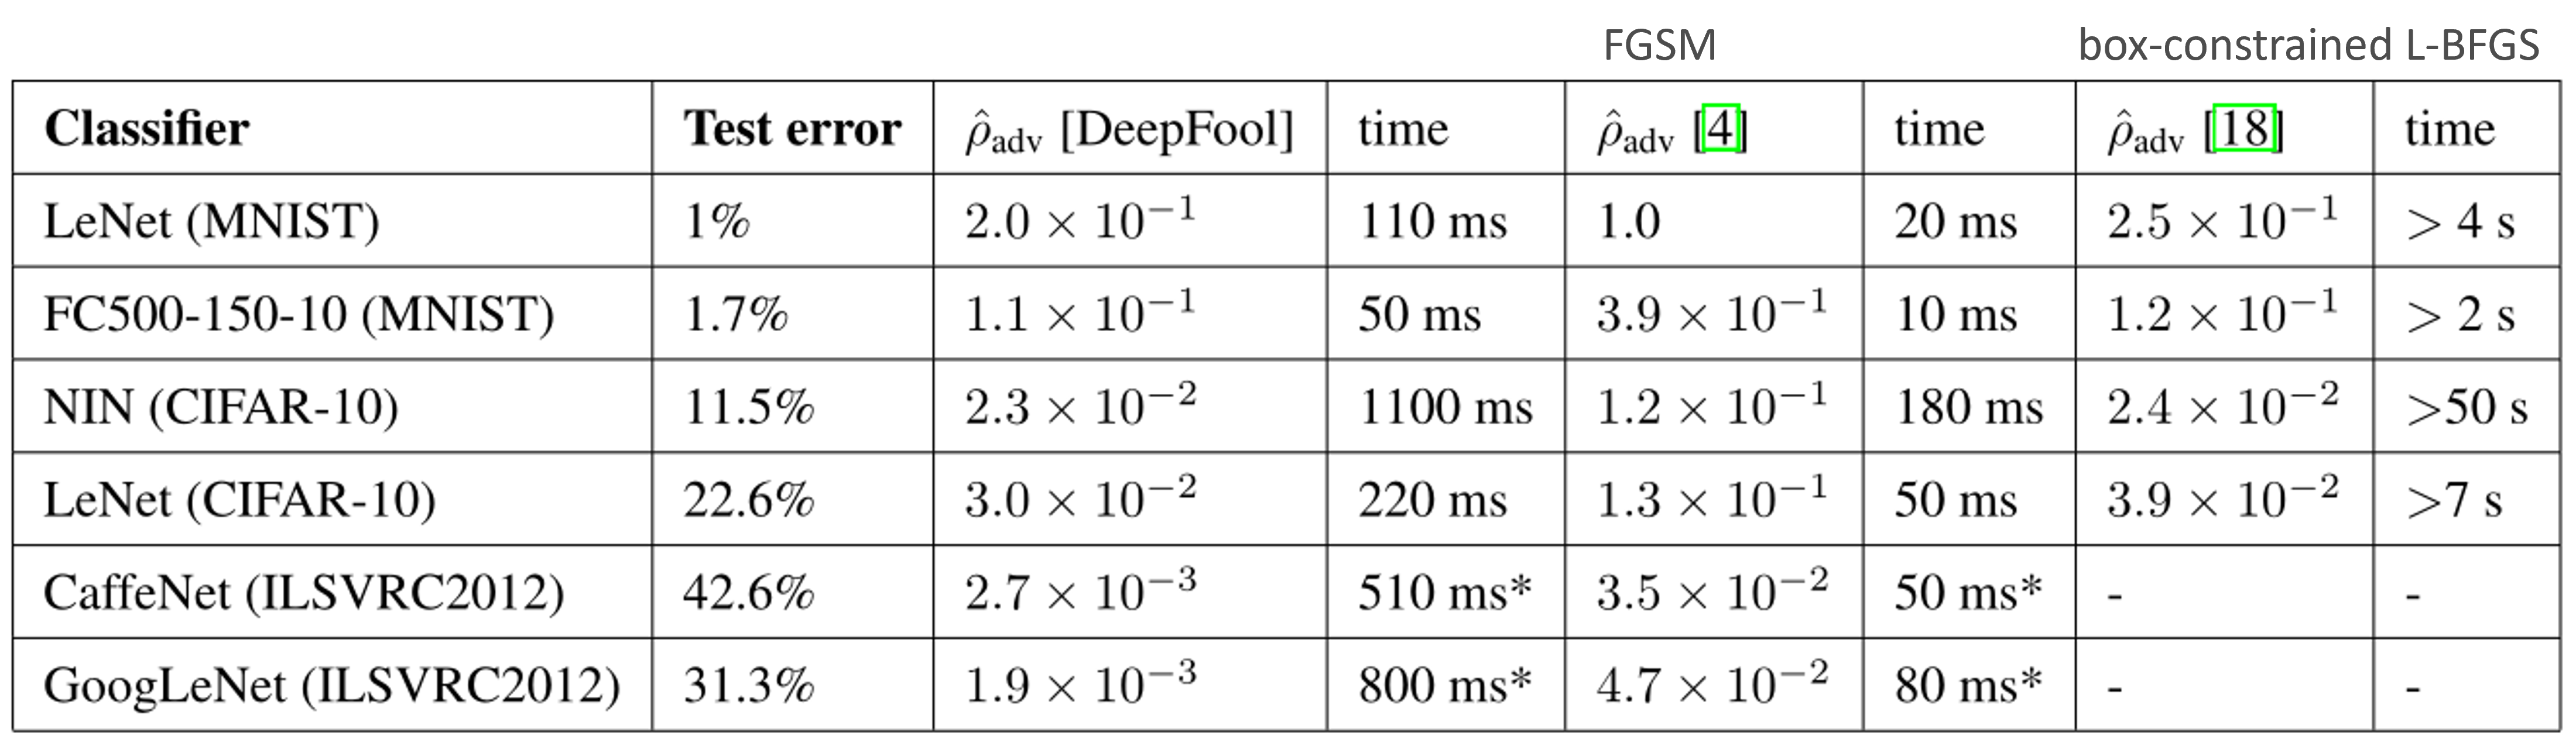
\includegraphics[width=0.9\textwidth]{docs/paperReading/deepfool/deepfool-result_1.png}
    \end{figure}
\end{frame}

\begin{frame}{DeepFool attack}
    \begin{figure}
        \centering
        \includegraphics[width=0.9\textwidth]{docs/paperReading/deepfool/deepfool-exp.png}
    \end{figure}
\end{frame}